% Created by tikzDevice version 0.8.1 on 2015-08-26 17:32:10
% !TEX encoding = UTF-8 Unicode
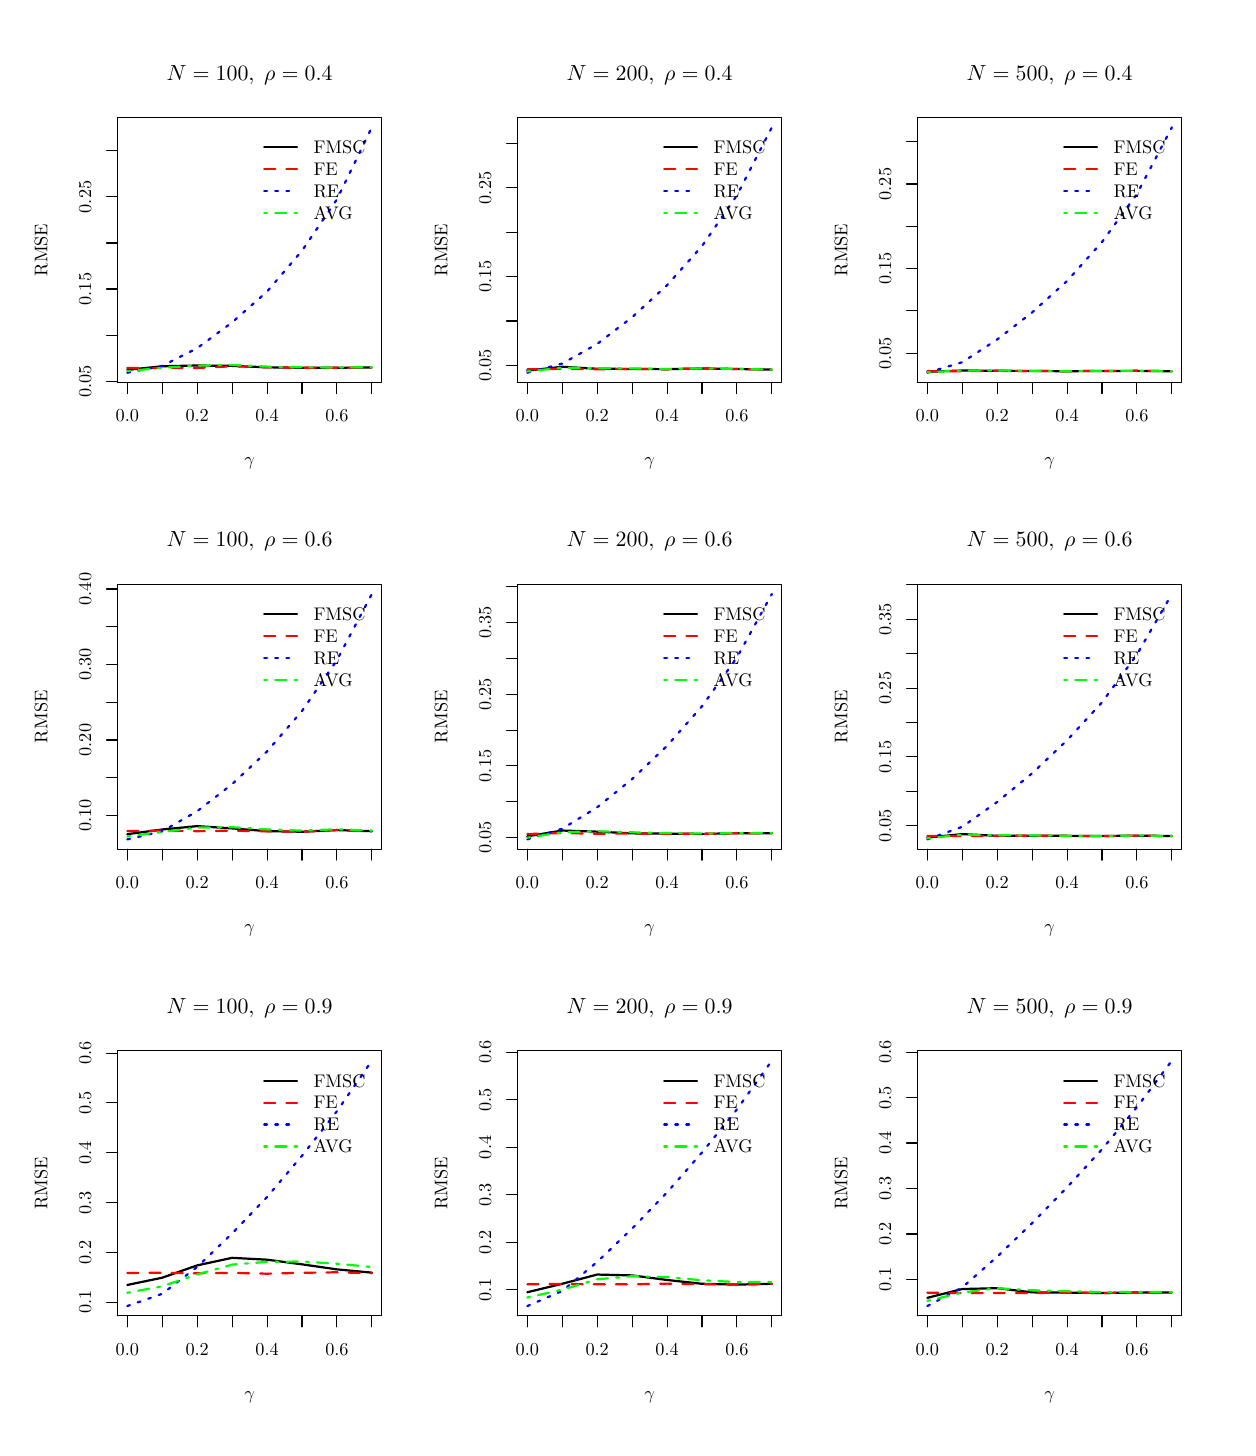
\begin{tikzpicture}[x=1pt,y=1pt]
\definecolor{fillColor}{RGB}{255,255,255}
\path[use as bounding box,fill=fillColor,fill opacity=0.00] (0,0) rectangle (433.62,505.89);
\begin{scope}
\path[clip] ( 32.47,377.65) rectangle (127.91,473.42);
\definecolor{drawColor}{RGB}{0,0,0}

\path[draw=drawColor,line width= 0.8pt,line join=round,line cap=round] ( 36.01,382.23) --
	( 48.63,383.54) --
	( 61.25,383.81) --
	( 73.88,383.67) --
	( 86.50,383.16) --
	( 99.13,382.97) --
	(111.75,383.02) --
	(124.37,383.08);
\end{scope}
\begin{scope}
\path[clip] (  0.00,  0.00) rectangle (433.62,505.89);
\definecolor{drawColor}{RGB}{0,0,0}

\path[draw=drawColor,line width= 0.4pt,line join=round,line cap=round] ( 36.01,377.65) -- (124.37,377.65);

\path[draw=drawColor,line width= 0.4pt,line join=round,line cap=round] ( 36.01,377.65) -- ( 36.01,373.69);

\path[draw=drawColor,line width= 0.4pt,line join=round,line cap=round] ( 48.63,377.65) -- ( 48.63,373.69);

\path[draw=drawColor,line width= 0.4pt,line join=round,line cap=round] ( 61.25,377.65) -- ( 61.25,373.69);

\path[draw=drawColor,line width= 0.4pt,line join=round,line cap=round] ( 73.88,377.65) -- ( 73.88,373.69);

\path[draw=drawColor,line width= 0.4pt,line join=round,line cap=round] ( 86.50,377.65) -- ( 86.50,373.69);

\path[draw=drawColor,line width= 0.4pt,line join=round,line cap=round] ( 99.13,377.65) -- ( 99.13,373.69);

\path[draw=drawColor,line width= 0.4pt,line join=round,line cap=round] (111.75,377.65) -- (111.75,373.69);

\path[draw=drawColor,line width= 0.4pt,line join=round,line cap=round] (124.37,377.65) -- (124.37,373.69);

\node[text=drawColor,anchor=base,inner sep=0pt, outer sep=0pt, scale=  0.66] at ( 36.01,363.40) {0.0};

\node[text=drawColor,anchor=base,inner sep=0pt, outer sep=0pt, scale=  0.66] at ( 61.25,363.40) {0.2};

\node[text=drawColor,anchor=base,inner sep=0pt, outer sep=0pt, scale=  0.66] at ( 86.50,363.40) {0.4};

\node[text=drawColor,anchor=base,inner sep=0pt, outer sep=0pt, scale=  0.66] at (111.75,363.40) {0.6};

\path[draw=drawColor,line width= 0.4pt,line join=round,line cap=round] ( 32.47,378.14) -- ( 32.47,461.37);

\path[draw=drawColor,line width= 0.4pt,line join=round,line cap=round] ( 32.47,378.14) -- ( 28.51,378.14);

\path[draw=drawColor,line width= 0.4pt,line join=round,line cap=round] ( 32.47,394.79) -- ( 28.51,394.79);

\path[draw=drawColor,line width= 0.4pt,line join=round,line cap=round] ( 32.47,411.44) -- ( 28.51,411.44);

\path[draw=drawColor,line width= 0.4pt,line join=round,line cap=round] ( 32.47,428.08) -- ( 28.51,428.08);

\path[draw=drawColor,line width= 0.4pt,line join=round,line cap=round] ( 32.47,444.73) -- ( 28.51,444.73);

\path[draw=drawColor,line width= 0.4pt,line join=round,line cap=round] ( 32.47,461.37) -- ( 28.51,461.37);

\node[text=drawColor,rotate= 90.00,anchor=base,inner sep=0pt, outer sep=0pt, scale=  0.66] at ( 22.97,378.14) {0.05};

\node[text=drawColor,rotate= 90.00,anchor=base,inner sep=0pt, outer sep=0pt, scale=  0.66] at ( 22.97,411.44) {0.15};

\node[text=drawColor,rotate= 90.00,anchor=base,inner sep=0pt, outer sep=0pt, scale=  0.66] at ( 22.97,444.73) {0.25};

\path[draw=drawColor,line width= 0.4pt,line join=round,line cap=round] ( 32.47,377.65) --
	(127.91,377.65) --
	(127.91,473.42) --
	( 32.47,473.42) --
	( 32.47,377.65);
\end{scope}
\begin{scope}
\path[clip] (  0.00,337.26) rectangle (144.54,505.89);
\definecolor{drawColor}{RGB}{0,0,0}

\node[text=drawColor,anchor=base,inner sep=0pt, outer sep=0pt, scale=  0.79] at ( 80.19,486.92) {\bfseries $N=100, \;\rho=0.4$};

\node[text=drawColor,anchor=base,inner sep=0pt, outer sep=0pt, scale=  0.66] at ( 80.19,347.56) {$\gamma$};

\node[text=drawColor,rotate= 90.00,anchor=base,inner sep=0pt, outer sep=0pt, scale=  0.66] at (  7.13,425.53) {RMSE};
\end{scope}
\begin{scope}
\path[clip] ( 32.47,377.65) rectangle (127.91,473.42);
\definecolor{drawColor}{RGB}{255,0,0}

\path[draw=drawColor,line width= 0.8pt,dash pattern=on 4pt off 4pt ,line join=round,line cap=round] ( 36.01,382.90) --
	( 48.63,382.93) --
	( 61.25,382.92) --
	( 73.88,383.53) --
	( 86.50,383.16) --
	( 99.13,382.97) --
	(111.75,383.02) --
	(124.37,383.08);
\definecolor{drawColor}{RGB}{0,0,255}

\path[draw=drawColor,line width= 0.8pt,dash pattern=on 1pt off 3pt ,line join=round,line cap=round] ( 36.01,381.20) --
	( 48.63,383.69) --
	( 61.25,390.07) --
	( 73.88,399.40) --
	( 86.50,410.52) --
	( 99.13,425.29) --
	(111.75,443.84) --
	(124.37,469.87);
\definecolor{drawColor}{RGB}{0,255,0}

\path[draw=drawColor,line width= 0.8pt,dash pattern=on 1pt off 3pt on 4pt off 3pt ,line join=round,line cap=round] ( 36.01,381.80) --
	( 48.63,382.98) --
	( 61.25,383.77) --
	( 73.88,384.04) --
	( 86.50,383.41) --
	( 99.13,383.13) --
	(111.75,383.12) --
	(124.37,383.16);
\definecolor{drawColor}{RGB}{0,0,0}

\path[draw=drawColor,line width= 0.8pt,line join=round,line cap=round] ( 85.47,462.63) -- ( 97.35,462.63);
\definecolor{drawColor}{RGB}{255,0,0}

\path[draw=drawColor,line width= 0.8pt,dash pattern=on 4pt off 4pt ,line join=round,line cap=round] ( 85.47,454.71) -- ( 97.35,454.71);
\definecolor{drawColor}{RGB}{0,0,255}

\path[draw=drawColor,line width= 0.8pt,dash pattern=on 1pt off 3pt ,line join=round,line cap=round] ( 85.47,446.79) -- ( 97.35,446.79);
\definecolor{drawColor}{RGB}{0,255,0}

\path[draw=drawColor,line width= 0.8pt,dash pattern=on 1pt off 3pt on 4pt off 3pt ,line join=round,line cap=round] ( 85.47,438.87) -- ( 97.35,438.87);
\definecolor{drawColor}{RGB}{0,0,0}

\node[text=drawColor,anchor=base west,inner sep=0pt, outer sep=0pt, scale=  0.66] at (103.29,460.35) {FMSC};

\node[text=drawColor,anchor=base west,inner sep=0pt, outer sep=0pt, scale=  0.66] at (103.29,452.43) {FE};

\node[text=drawColor,anchor=base west,inner sep=0pt, outer sep=0pt, scale=  0.66] at (103.29,444.51) {RE};

\node[text=drawColor,anchor=base west,inner sep=0pt, outer sep=0pt, scale=  0.66] at (103.29,436.59) {AVG};
\end{scope}
\begin{scope}
\path[clip] (177.01,377.65) rectangle (272.45,473.42);
\definecolor{drawColor}{RGB}{0,0,0}

\path[draw=drawColor,line width= 0.8pt,line join=round,line cap=round] (180.55,381.97) --
	(193.17,383.35) --
	(205.79,382.63) --
	(218.42,382.57) --
	(231.04,382.48) --
	(243.67,382.74) --
	(256.29,382.55) --
	(268.91,382.32);
\end{scope}
\begin{scope}
\path[clip] (  0.00,  0.00) rectangle (433.62,505.89);
\definecolor{drawColor}{RGB}{0,0,0}

\path[draw=drawColor,line width= 0.4pt,line join=round,line cap=round] (180.55,377.65) -- (268.91,377.65);

\path[draw=drawColor,line width= 0.4pt,line join=round,line cap=round] (180.55,377.65) -- (180.55,373.69);

\path[draw=drawColor,line width= 0.4pt,line join=round,line cap=round] (193.17,377.65) -- (193.17,373.69);

\path[draw=drawColor,line width= 0.4pt,line join=round,line cap=round] (205.79,377.65) -- (205.79,373.69);

\path[draw=drawColor,line width= 0.4pt,line join=round,line cap=round] (218.42,377.65) -- (218.42,373.69);

\path[draw=drawColor,line width= 0.4pt,line join=round,line cap=round] (231.04,377.65) -- (231.04,373.69);

\path[draw=drawColor,line width= 0.4pt,line join=round,line cap=round] (243.67,377.65) -- (243.67,373.69);

\path[draw=drawColor,line width= 0.4pt,line join=round,line cap=round] (256.29,377.65) -- (256.29,373.69);

\path[draw=drawColor,line width= 0.4pt,line join=round,line cap=round] (268.91,377.65) -- (268.91,373.69);

\node[text=drawColor,anchor=base,inner sep=0pt, outer sep=0pt, scale=  0.66] at (180.55,363.40) {0.0};

\node[text=drawColor,anchor=base,inner sep=0pt, outer sep=0pt, scale=  0.66] at (205.79,363.40) {0.2};

\node[text=drawColor,anchor=base,inner sep=0pt, outer sep=0pt, scale=  0.66] at (231.04,363.40) {0.4};

\node[text=drawColor,anchor=base,inner sep=0pt, outer sep=0pt, scale=  0.66] at (256.29,363.40) {0.6};

\path[draw=drawColor,line width= 0.4pt,line join=round,line cap=round] (177.01,383.89) -- (177.01,464.00);

\path[draw=drawColor,line width= 0.4pt,line join=round,line cap=round] (177.01,383.89) -- (173.05,383.89);

\path[draw=drawColor,line width= 0.4pt,line join=round,line cap=round] (177.01,399.91) -- (173.05,399.91);

\path[draw=drawColor,line width= 0.4pt,line join=round,line cap=round] (177.01,415.94) -- (173.05,415.94);

\path[draw=drawColor,line width= 0.4pt,line join=round,line cap=round] (177.01,431.96) -- (173.05,431.96);

\path[draw=drawColor,line width= 0.4pt,line join=round,line cap=round] (177.01,447.98) -- (173.05,447.98);

\path[draw=drawColor,line width= 0.4pt,line join=round,line cap=round] (177.01,464.00) -- (173.05,464.00);

\node[text=drawColor,rotate= 90.00,anchor=base,inner sep=0pt, outer sep=0pt, scale=  0.66] at (167.51,383.89) {0.05};

\node[text=drawColor,rotate= 90.00,anchor=base,inner sep=0pt, outer sep=0pt, scale=  0.66] at (167.51,415.94) {0.15};

\node[text=drawColor,rotate= 90.00,anchor=base,inner sep=0pt, outer sep=0pt, scale=  0.66] at (167.51,447.98) {0.25};

\path[draw=drawColor,line width= 0.4pt,line join=round,line cap=round] (177.01,377.65) --
	(272.45,377.65) --
	(272.45,473.42) --
	(177.01,473.42) --
	(177.01,377.65);
\end{scope}
\begin{scope}
\path[clip] (144.54,337.26) rectangle (289.08,505.89);
\definecolor{drawColor}{RGB}{0,0,0}

\node[text=drawColor,anchor=base,inner sep=0pt, outer sep=0pt, scale=  0.79] at (224.73,486.92) {\bfseries $N=200, \;\rho=0.4$};

\node[text=drawColor,anchor=base,inner sep=0pt, outer sep=0pt, scale=  0.66] at (224.73,347.56) {$\gamma$};

\node[text=drawColor,rotate= 90.00,anchor=base,inner sep=0pt, outer sep=0pt, scale=  0.66] at (151.67,425.53) {RMSE};
\end{scope}
\begin{scope}
\path[clip] (177.01,377.65) rectangle (272.45,473.42);
\definecolor{drawColor}{RGB}{255,0,0}

\path[draw=drawColor,line width= 0.8pt,dash pattern=on 4pt off 4pt ,line join=round,line cap=round] (180.55,382.44) --
	(193.17,382.62) --
	(205.79,382.45) --
	(218.42,382.57) --
	(231.04,382.48) --
	(243.67,382.74) --
	(256.29,382.55) --
	(268.91,382.32);
\definecolor{drawColor}{RGB}{0,0,255}

\path[draw=drawColor,line width= 0.8pt,dash pattern=on 1pt off 3pt ,line join=round,line cap=round] (180.55,381.20) --
	(193.17,384.51) --
	(205.79,391.60) --
	(218.42,401.26) --
	(231.04,412.83) --
	(243.67,426.96) --
	(256.29,445.31) --
	(268.91,469.87);
\definecolor{drawColor}{RGB}{0,255,0}

\path[draw=drawColor,line width= 0.8pt,dash pattern=on 1pt off 3pt on 4pt off 3pt ,line join=round,line cap=round] (180.55,381.67) --
	(193.17,383.02) --
	(205.79,382.87) --
	(218.42,382.73) --
	(231.04,382.57) --
	(243.67,382.79) --
	(256.29,382.58) --
	(268.91,382.33);
\definecolor{drawColor}{RGB}{0,0,0}

\path[draw=drawColor,line width= 0.8pt,line join=round,line cap=round] (230.01,462.63) -- (241.89,462.63);
\definecolor{drawColor}{RGB}{255,0,0}

\path[draw=drawColor,line width= 0.8pt,dash pattern=on 4pt off 4pt ,line join=round,line cap=round] (230.01,454.71) -- (241.89,454.71);
\definecolor{drawColor}{RGB}{0,0,255}

\path[draw=drawColor,line width= 0.8pt,dash pattern=on 1pt off 3pt ,line join=round,line cap=round] (230.01,446.79) -- (241.89,446.79);
\definecolor{drawColor}{RGB}{0,255,0}

\path[draw=drawColor,line width= 0.8pt,dash pattern=on 1pt off 3pt on 4pt off 3pt ,line join=round,line cap=round] (230.01,438.87) -- (241.89,438.87);
\definecolor{drawColor}{RGB}{0,0,0}

\node[text=drawColor,anchor=base west,inner sep=0pt, outer sep=0pt, scale=  0.66] at (247.83,460.35) {FMSC};

\node[text=drawColor,anchor=base west,inner sep=0pt, outer sep=0pt, scale=  0.66] at (247.83,452.43) {FE};

\node[text=drawColor,anchor=base west,inner sep=0pt, outer sep=0pt, scale=  0.66] at (247.83,444.51) {RE};

\node[text=drawColor,anchor=base west,inner sep=0pt, outer sep=0pt, scale=  0.66] at (247.83,436.59) {AVG};
\end{scope}
\begin{scope}
\path[clip] (321.55,377.65) rectangle (416.99,473.42);
\definecolor{drawColor}{RGB}{0,0,0}

\path[draw=drawColor,line width= 0.8pt,line join=round,line cap=round] (325.09,381.55) --
	(337.71,382.01) --
	(350.33,381.91) --
	(362.96,381.83) --
	(375.58,381.74) --
	(388.21,381.84) --
	(400.83,381.88) --
	(413.45,381.73);
\end{scope}
\begin{scope}
\path[clip] (  0.00,  0.00) rectangle (433.62,505.89);
\definecolor{drawColor}{RGB}{0,0,0}

\path[draw=drawColor,line width= 0.4pt,line join=round,line cap=round] (325.09,377.65) -- (413.45,377.65);

\path[draw=drawColor,line width= 0.4pt,line join=round,line cap=round] (325.09,377.65) -- (325.09,373.69);

\path[draw=drawColor,line width= 0.4pt,line join=round,line cap=round] (337.71,377.65) -- (337.71,373.69);

\path[draw=drawColor,line width= 0.4pt,line join=round,line cap=round] (350.33,377.65) -- (350.33,373.69);

\path[draw=drawColor,line width= 0.4pt,line join=round,line cap=round] (362.96,377.65) -- (362.96,373.69);

\path[draw=drawColor,line width= 0.4pt,line join=round,line cap=round] (375.58,377.65) -- (375.58,373.69);

\path[draw=drawColor,line width= 0.4pt,line join=round,line cap=round] (388.21,377.65) -- (388.21,373.69);

\path[draw=drawColor,line width= 0.4pt,line join=round,line cap=round] (400.83,377.65) -- (400.83,373.69);

\path[draw=drawColor,line width= 0.4pt,line join=round,line cap=round] (413.45,377.65) -- (413.45,373.69);

\node[text=drawColor,anchor=base,inner sep=0pt, outer sep=0pt, scale=  0.66] at (325.09,363.40) {0.0};

\node[text=drawColor,anchor=base,inner sep=0pt, outer sep=0pt, scale=  0.66] at (350.33,363.40) {0.2};

\node[text=drawColor,anchor=base,inner sep=0pt, outer sep=0pt, scale=  0.66] at (375.58,363.40) {0.4};

\node[text=drawColor,anchor=base,inner sep=0pt, outer sep=0pt, scale=  0.66] at (400.83,363.40) {0.6};

\path[draw=drawColor,line width= 0.4pt,line join=round,line cap=round] (321.55,388.28) -- (321.55,464.66);

\path[draw=drawColor,line width= 0.4pt,line join=round,line cap=round] (321.55,388.28) -- (317.59,388.28);

\path[draw=drawColor,line width= 0.4pt,line join=round,line cap=round] (321.55,403.55) -- (317.59,403.55);

\path[draw=drawColor,line width= 0.4pt,line join=round,line cap=round] (321.55,418.83) -- (317.59,418.83);

\path[draw=drawColor,line width= 0.4pt,line join=round,line cap=round] (321.55,434.10) -- (317.59,434.10);

\path[draw=drawColor,line width= 0.4pt,line join=round,line cap=round] (321.55,449.38) -- (317.59,449.38);

\path[draw=drawColor,line width= 0.4pt,line join=round,line cap=round] (321.55,464.66) -- (317.59,464.66);

\node[text=drawColor,rotate= 90.00,anchor=base,inner sep=0pt, outer sep=0pt, scale=  0.66] at (312.05,388.28) {0.05};

\node[text=drawColor,rotate= 90.00,anchor=base,inner sep=0pt, outer sep=0pt, scale=  0.66] at (312.05,418.83) {0.15};

\node[text=drawColor,rotate= 90.00,anchor=base,inner sep=0pt, outer sep=0pt, scale=  0.66] at (312.05,449.38) {0.25};

\path[draw=drawColor,line width= 0.4pt,line join=round,line cap=round] (321.55,377.65) --
	(416.99,377.65) --
	(416.99,473.42) --
	(321.55,473.42) --
	(321.55,377.65);
\end{scope}
\begin{scope}
\path[clip] (289.08,337.26) rectangle (433.62,505.89);
\definecolor{drawColor}{RGB}{0,0,0}

\node[text=drawColor,anchor=base,inner sep=0pt, outer sep=0pt, scale=  0.79] at (369.27,486.92) {\bfseries $N=500, \;\rho=0.4$};

\node[text=drawColor,anchor=base,inner sep=0pt, outer sep=0pt, scale=  0.66] at (369.27,347.56) {$\gamma$};

\node[text=drawColor,rotate= 90.00,anchor=base,inner sep=0pt, outer sep=0pt, scale=  0.66] at (296.21,425.53) {RMSE};
\end{scope}
\begin{scope}
\path[clip] (321.55,377.65) rectangle (416.99,473.42);
\definecolor{drawColor}{RGB}{255,0,0}

\path[draw=drawColor,line width= 0.8pt,dash pattern=on 4pt off 4pt ,line join=round,line cap=round] (325.09,381.79) --
	(337.71,381.72) --
	(350.33,381.91) --
	(362.96,381.83) --
	(375.58,381.74) --
	(388.21,381.84) --
	(400.83,381.88) --
	(413.45,381.73);
\definecolor{drawColor}{RGB}{0,0,255}

\path[draw=drawColor,line width= 0.8pt,dash pattern=on 1pt off 3pt ,line join=round,line cap=round] (325.09,381.20) --
	(337.71,385.00) --
	(350.33,393.22) --
	(362.96,402.99) --
	(375.58,414.35) --
	(388.21,428.45) --
	(400.83,445.80) --
	(413.45,469.87);
\definecolor{drawColor}{RGB}{0,255,0}

\path[draw=drawColor,line width= 0.8pt,dash pattern=on 1pt off 3pt on 4pt off 3pt ,line join=round,line cap=round] (325.09,381.38) --
	(337.71,382.01) --
	(350.33,381.99) --
	(362.96,381.87) --
	(375.58,381.76) --
	(388.21,381.85) --
	(400.83,381.88) --
	(413.45,381.73);
\definecolor{drawColor}{RGB}{0,0,0}

\path[draw=drawColor,line width= 0.8pt,line join=round,line cap=round] (374.55,462.63) -- (386.43,462.63);
\definecolor{drawColor}{RGB}{255,0,0}

\path[draw=drawColor,line width= 0.8pt,dash pattern=on 4pt off 4pt ,line join=round,line cap=round] (374.55,454.71) -- (386.43,454.71);
\definecolor{drawColor}{RGB}{0,0,255}

\path[draw=drawColor,line width= 0.8pt,dash pattern=on 1pt off 3pt ,line join=round,line cap=round] (374.55,446.79) -- (386.43,446.79);
\definecolor{drawColor}{RGB}{0,255,0}

\path[draw=drawColor,line width= 0.8pt,dash pattern=on 1pt off 3pt on 4pt off 3pt ,line join=round,line cap=round] (374.55,438.87) -- (386.43,438.87);
\definecolor{drawColor}{RGB}{0,0,0}

\node[text=drawColor,anchor=base west,inner sep=0pt, outer sep=0pt, scale=  0.66] at (392.37,460.35) {FMSC};

\node[text=drawColor,anchor=base west,inner sep=0pt, outer sep=0pt, scale=  0.66] at (392.37,452.43) {FE};

\node[text=drawColor,anchor=base west,inner sep=0pt, outer sep=0pt, scale=  0.66] at (392.37,444.51) {RE};

\node[text=drawColor,anchor=base west,inner sep=0pt, outer sep=0pt, scale=  0.66] at (392.37,436.59) {AVG};
\end{scope}
\begin{scope}
\path[clip] ( 32.47,209.02) rectangle (127.91,304.79);
\definecolor{drawColor}{RGB}{0,0,0}

\path[draw=drawColor,line width= 0.8pt,line join=round,line cap=round] ( 36.01,214.46) --
	( 48.63,216.15) --
	( 61.25,217.37) --
	( 73.88,216.54) --
	( 86.50,215.55) --
	( 99.13,215.34) --
	(111.75,215.94) --
	(124.37,215.53);
\end{scope}
\begin{scope}
\path[clip] (  0.00,  0.00) rectangle (433.62,505.89);
\definecolor{drawColor}{RGB}{0,0,0}

\path[draw=drawColor,line width= 0.4pt,line join=round,line cap=round] ( 36.01,209.02) -- (124.37,209.02);

\path[draw=drawColor,line width= 0.4pt,line join=round,line cap=round] ( 36.01,209.02) -- ( 36.01,205.06);

\path[draw=drawColor,line width= 0.4pt,line join=round,line cap=round] ( 48.63,209.02) -- ( 48.63,205.06);

\path[draw=drawColor,line width= 0.4pt,line join=round,line cap=round] ( 61.25,209.02) -- ( 61.25,205.06);

\path[draw=drawColor,line width= 0.4pt,line join=round,line cap=round] ( 73.88,209.02) -- ( 73.88,205.06);

\path[draw=drawColor,line width= 0.4pt,line join=round,line cap=round] ( 86.50,209.02) -- ( 86.50,205.06);

\path[draw=drawColor,line width= 0.4pt,line join=round,line cap=round] ( 99.13,209.02) -- ( 99.13,205.06);

\path[draw=drawColor,line width= 0.4pt,line join=round,line cap=round] (111.75,209.02) -- (111.75,205.06);

\path[draw=drawColor,line width= 0.4pt,line join=round,line cap=round] (124.37,209.02) -- (124.37,205.06);

\node[text=drawColor,anchor=base,inner sep=0pt, outer sep=0pt, scale=  0.66] at ( 36.01,194.77) {0.0};

\node[text=drawColor,anchor=base,inner sep=0pt, outer sep=0pt, scale=  0.66] at ( 61.25,194.77) {0.2};

\node[text=drawColor,anchor=base,inner sep=0pt, outer sep=0pt, scale=  0.66] at ( 86.50,194.77) {0.4};

\node[text=drawColor,anchor=base,inner sep=0pt, outer sep=0pt, scale=  0.66] at (111.75,194.77) {0.6};

\path[draw=drawColor,line width= 0.4pt,line join=round,line cap=round] ( 32.47,221.21) -- ( 32.47,303.04);

\path[draw=drawColor,line width= 0.4pt,line join=round,line cap=round] ( 32.47,221.21) -- ( 28.51,221.21);

\path[draw=drawColor,line width= 0.4pt,line join=round,line cap=round] ( 32.47,234.85) -- ( 28.51,234.85);

\path[draw=drawColor,line width= 0.4pt,line join=round,line cap=round] ( 32.47,248.49) -- ( 28.51,248.49);

\path[draw=drawColor,line width= 0.4pt,line join=round,line cap=round] ( 32.47,262.12) -- ( 28.51,262.12);

\path[draw=drawColor,line width= 0.4pt,line join=round,line cap=round] ( 32.47,275.76) -- ( 28.51,275.76);

\path[draw=drawColor,line width= 0.4pt,line join=round,line cap=round] ( 32.47,289.40) -- ( 28.51,289.40);

\path[draw=drawColor,line width= 0.4pt,line join=round,line cap=round] ( 32.47,303.04) -- ( 28.51,303.04);

\node[text=drawColor,rotate= 90.00,anchor=base,inner sep=0pt, outer sep=0pt, scale=  0.66] at ( 22.97,221.21) {0.10};

\node[text=drawColor,rotate= 90.00,anchor=base,inner sep=0pt, outer sep=0pt, scale=  0.66] at ( 22.97,248.49) {0.20};

\node[text=drawColor,rotate= 90.00,anchor=base,inner sep=0pt, outer sep=0pt, scale=  0.66] at ( 22.97,275.76) {0.30};

\node[text=drawColor,rotate= 90.00,anchor=base,inner sep=0pt, outer sep=0pt, scale=  0.66] at ( 22.97,303.04) {0.40};

\path[draw=drawColor,line width= 0.4pt,line join=round,line cap=round] ( 32.47,209.02) --
	(127.91,209.02) --
	(127.91,304.79) --
	( 32.47,304.79) --
	( 32.47,209.02);
\end{scope}
\begin{scope}
\path[clip] (  0.00,168.63) rectangle (144.54,337.26);
\definecolor{drawColor}{RGB}{0,0,0}

\node[text=drawColor,anchor=base,inner sep=0pt, outer sep=0pt, scale=  0.79] at ( 80.19,318.29) {\bfseries $N=100, \;\rho=0.6$};

\node[text=drawColor,anchor=base,inner sep=0pt, outer sep=0pt, scale=  0.66] at ( 80.19,178.93) {$\gamma$};

\node[text=drawColor,rotate= 90.00,anchor=base,inner sep=0pt, outer sep=0pt, scale=  0.66] at (  7.13,256.90) {RMSE};
\end{scope}
\begin{scope}
\path[clip] ( 32.47,209.02) rectangle (127.91,304.79);
\definecolor{drawColor}{RGB}{255,0,0}

\path[draw=drawColor,line width= 0.8pt,dash pattern=on 4pt off 4pt ,line join=round,line cap=round] ( 36.01,215.59) --
	( 48.63,215.77) --
	( 61.25,215.54) --
	( 73.88,215.72) --
	( 86.50,215.48) --
	( 99.13,215.34) --
	(111.75,215.94) --
	(124.37,215.53);
\definecolor{drawColor}{RGB}{0,0,255}

\path[draw=drawColor,line width= 0.8pt,dash pattern=on 1pt off 3pt ,line join=round,line cap=round] ( 36.01,212.57) --
	( 48.63,215.51) --
	( 61.25,222.75) --
	( 73.88,232.53) --
	( 86.50,244.35) --
	( 99.13,258.98) --
	(111.75,277.36) --
	(124.37,301.24);
\definecolor{drawColor}{RGB}{0,255,0}

\path[draw=drawColor,line width= 0.8pt,dash pattern=on 1pt off 3pt on 4pt off 3pt ,line join=round,line cap=round] ( 36.01,213.65) --
	( 48.63,215.24) --
	( 61.25,216.84) --
	( 73.88,216.97) --
	( 86.50,216.19) --
	( 99.13,215.75) --
	(111.75,216.23) --
	(124.37,215.74);
\definecolor{drawColor}{RGB}{0,0,0}

\path[draw=drawColor,line width= 0.8pt,line join=round,line cap=round] ( 85.47,294.00) -- ( 97.35,294.00);
\definecolor{drawColor}{RGB}{255,0,0}

\path[draw=drawColor,line width= 0.8pt,dash pattern=on 4pt off 4pt ,line join=round,line cap=round] ( 85.47,286.08) -- ( 97.35,286.08);
\definecolor{drawColor}{RGB}{0,0,255}

\path[draw=drawColor,line width= 0.8pt,dash pattern=on 1pt off 3pt ,line join=round,line cap=round] ( 85.47,278.16) -- ( 97.35,278.16);
\definecolor{drawColor}{RGB}{0,255,0}

\path[draw=drawColor,line width= 0.8pt,dash pattern=on 1pt off 3pt on 4pt off 3pt ,line join=round,line cap=round] ( 85.47,270.24) -- ( 97.35,270.24);
\definecolor{drawColor}{RGB}{0,0,0}

\node[text=drawColor,anchor=base west,inner sep=0pt, outer sep=0pt, scale=  0.66] at (103.29,291.72) {FMSC};

\node[text=drawColor,anchor=base west,inner sep=0pt, outer sep=0pt, scale=  0.66] at (103.29,283.80) {FE};

\node[text=drawColor,anchor=base west,inner sep=0pt, outer sep=0pt, scale=  0.66] at (103.29,275.88) {RE};

\node[text=drawColor,anchor=base west,inner sep=0pt, outer sep=0pt, scale=  0.66] at (103.29,267.96) {AVG};
\end{scope}
\begin{scope}
\path[clip] (177.01,209.02) rectangle (272.45,304.79);
\definecolor{drawColor}{RGB}{0,0,0}

\path[draw=drawColor,line width= 0.8pt,line join=round,line cap=round] (180.55,213.68) --
	(193.17,215.77) --
	(205.79,215.37) --
	(218.42,214.75) --
	(231.04,214.64) --
	(243.67,214.55) --
	(256.29,214.80) --
	(268.91,214.83);
\end{scope}
\begin{scope}
\path[clip] (  0.00,  0.00) rectangle (433.62,505.89);
\definecolor{drawColor}{RGB}{0,0,0}

\path[draw=drawColor,line width= 0.4pt,line join=round,line cap=round] (180.55,209.02) -- (268.91,209.02);

\path[draw=drawColor,line width= 0.4pt,line join=round,line cap=round] (180.55,209.02) -- (180.55,205.06);

\path[draw=drawColor,line width= 0.4pt,line join=round,line cap=round] (193.17,209.02) -- (193.17,205.06);

\path[draw=drawColor,line width= 0.4pt,line join=round,line cap=round] (205.79,209.02) -- (205.79,205.06);

\path[draw=drawColor,line width= 0.4pt,line join=round,line cap=round] (218.42,209.02) -- (218.42,205.06);

\path[draw=drawColor,line width= 0.4pt,line join=round,line cap=round] (231.04,209.02) -- (231.04,205.06);

\path[draw=drawColor,line width= 0.4pt,line join=round,line cap=round] (243.67,209.02) -- (243.67,205.06);

\path[draw=drawColor,line width= 0.4pt,line join=round,line cap=round] (256.29,209.02) -- (256.29,205.06);

\path[draw=drawColor,line width= 0.4pt,line join=round,line cap=round] (268.91,209.02) -- (268.91,205.06);

\node[text=drawColor,anchor=base,inner sep=0pt, outer sep=0pt, scale=  0.66] at (180.55,194.77) {0.0};

\node[text=drawColor,anchor=base,inner sep=0pt, outer sep=0pt, scale=  0.66] at (205.79,194.77) {0.2};

\node[text=drawColor,anchor=base,inner sep=0pt, outer sep=0pt, scale=  0.66] at (231.04,194.77) {0.4};

\node[text=drawColor,anchor=base,inner sep=0pt, outer sep=0pt, scale=  0.66] at (256.29,194.77) {0.6};

\path[draw=drawColor,line width= 0.4pt,line join=round,line cap=round] (177.01,213.18) -- (177.01,303.95);

\path[draw=drawColor,line width= 0.4pt,line join=round,line cap=round] (177.01,213.18) -- (173.05,213.18);

\path[draw=drawColor,line width= 0.4pt,line join=round,line cap=round] (177.01,226.15) -- (173.05,226.15);

\path[draw=drawColor,line width= 0.4pt,line join=round,line cap=round] (177.01,239.12) -- (173.05,239.12);

\path[draw=drawColor,line width= 0.4pt,line join=round,line cap=round] (177.01,252.08) -- (173.05,252.08);

\path[draw=drawColor,line width= 0.4pt,line join=round,line cap=round] (177.01,265.05) -- (173.05,265.05);

\path[draw=drawColor,line width= 0.4pt,line join=round,line cap=round] (177.01,278.02) -- (173.05,278.02);

\path[draw=drawColor,line width= 0.4pt,line join=round,line cap=round] (177.01,290.98) -- (173.05,290.98);

\path[draw=drawColor,line width= 0.4pt,line join=round,line cap=round] (177.01,303.95) -- (173.05,303.95);

\node[text=drawColor,rotate= 90.00,anchor=base,inner sep=0pt, outer sep=0pt, scale=  0.66] at (167.51,213.18) {0.05};

\node[text=drawColor,rotate= 90.00,anchor=base,inner sep=0pt, outer sep=0pt, scale=  0.66] at (167.51,239.12) {0.15};

\node[text=drawColor,rotate= 90.00,anchor=base,inner sep=0pt, outer sep=0pt, scale=  0.66] at (167.51,265.05) {0.25};

\node[text=drawColor,rotate= 90.00,anchor=base,inner sep=0pt, outer sep=0pt, scale=  0.66] at (167.51,290.98) {0.35};

\path[draw=drawColor,line width= 0.4pt,line join=round,line cap=round] (177.01,209.02) --
	(272.45,209.02) --
	(272.45,304.79) --
	(177.01,304.79) --
	(177.01,209.02);
\end{scope}
\begin{scope}
\path[clip] (144.54,168.63) rectangle (289.08,337.26);
\definecolor{drawColor}{RGB}{0,0,0}

\node[text=drawColor,anchor=base,inner sep=0pt, outer sep=0pt, scale=  0.79] at (224.73,318.29) {\bfseries $N=200, \;\rho=0.6$};

\node[text=drawColor,anchor=base,inner sep=0pt, outer sep=0pt, scale=  0.66] at (224.73,178.93) {$\gamma$};

\node[text=drawColor,rotate= 90.00,anchor=base,inner sep=0pt, outer sep=0pt, scale=  0.66] at (151.67,256.90) {RMSE};
\end{scope}
\begin{scope}
\path[clip] (177.01,209.02) rectangle (272.45,304.79);
\definecolor{drawColor}{RGB}{255,0,0}

\path[draw=drawColor,line width= 0.8pt,dash pattern=on 4pt off 4pt ,line join=round,line cap=round] (180.55,214.51) --
	(193.17,214.87) --
	(205.79,214.61) --
	(218.42,214.70) --
	(231.04,214.64) --
	(243.67,214.55) --
	(256.29,214.80) --
	(268.91,214.83);
\definecolor{drawColor}{RGB}{0,0,255}

\path[draw=drawColor,line width= 0.8pt,dash pattern=on 1pt off 3pt ,line join=round,line cap=round] (180.55,212.57) --
	(193.17,216.43) --
	(205.79,224.17) --
	(218.42,234.36) --
	(231.04,246.38) --
	(243.67,260.69) --
	(256.29,278.31) --
	(268.91,301.24);
\definecolor{drawColor}{RGB}{0,255,0}

\path[draw=drawColor,line width= 0.8pt,dash pattern=on 1pt off 3pt on 4pt off 3pt ,line join=round,line cap=round] (180.55,213.19) --
	(193.17,215.16) --
	(205.79,215.51) --
	(218.42,215.13) --
	(231.04,214.86) --
	(243.67,214.67) --
	(256.29,214.90) --
	(268.91,214.90);
\definecolor{drawColor}{RGB}{0,0,0}

\path[draw=drawColor,line width= 0.8pt,line join=round,line cap=round] (230.01,294.00) -- (241.89,294.00);
\definecolor{drawColor}{RGB}{255,0,0}

\path[draw=drawColor,line width= 0.8pt,dash pattern=on 4pt off 4pt ,line join=round,line cap=round] (230.01,286.08) -- (241.89,286.08);
\definecolor{drawColor}{RGB}{0,0,255}

\path[draw=drawColor,line width= 0.8pt,dash pattern=on 1pt off 3pt ,line join=round,line cap=round] (230.01,278.16) -- (241.89,278.16);
\definecolor{drawColor}{RGB}{0,255,0}

\path[draw=drawColor,line width= 0.8pt,dash pattern=on 1pt off 3pt on 4pt off 3pt ,line join=round,line cap=round] (230.01,270.24) -- (241.89,270.24);
\definecolor{drawColor}{RGB}{0,0,0}

\node[text=drawColor,anchor=base west,inner sep=0pt, outer sep=0pt, scale=  0.66] at (247.83,291.72) {FMSC};

\node[text=drawColor,anchor=base west,inner sep=0pt, outer sep=0pt, scale=  0.66] at (247.83,283.80) {FE};

\node[text=drawColor,anchor=base west,inner sep=0pt, outer sep=0pt, scale=  0.66] at (247.83,275.88) {RE};

\node[text=drawColor,anchor=base west,inner sep=0pt, outer sep=0pt, scale=  0.66] at (247.83,267.96) {AVG};
\end{scope}
\begin{scope}
\path[clip] (321.55,209.02) rectangle (416.99,304.79);
\definecolor{drawColor}{RGB}{0,0,0}

\path[draw=drawColor,line width= 0.8pt,line join=round,line cap=round] (325.09,213.24) --
	(337.71,214.48) --
	(350.33,213.86) --
	(362.96,213.90) --
	(375.58,213.85) --
	(388.21,213.78) --
	(400.83,213.94) --
	(413.45,213.77);
\end{scope}
\begin{scope}
\path[clip] (  0.00,  0.00) rectangle (433.62,505.89);
\definecolor{drawColor}{RGB}{0,0,0}

\path[draw=drawColor,line width= 0.4pt,line join=round,line cap=round] (325.09,209.02) -- (413.45,209.02);

\path[draw=drawColor,line width= 0.4pt,line join=round,line cap=round] (325.09,209.02) -- (325.09,205.06);

\path[draw=drawColor,line width= 0.4pt,line join=round,line cap=round] (337.71,209.02) -- (337.71,205.06);

\path[draw=drawColor,line width= 0.4pt,line join=round,line cap=round] (350.33,209.02) -- (350.33,205.06);

\path[draw=drawColor,line width= 0.4pt,line join=round,line cap=round] (362.96,209.02) -- (362.96,205.06);

\path[draw=drawColor,line width= 0.4pt,line join=round,line cap=round] (375.58,209.02) -- (375.58,205.06);

\path[draw=drawColor,line width= 0.4pt,line join=round,line cap=round] (388.21,209.02) -- (388.21,205.06);

\path[draw=drawColor,line width= 0.4pt,line join=round,line cap=round] (400.83,209.02) -- (400.83,205.06);

\path[draw=drawColor,line width= 0.4pt,line join=round,line cap=round] (413.45,209.02) -- (413.45,205.06);

\node[text=drawColor,anchor=base,inner sep=0pt, outer sep=0pt, scale=  0.66] at (325.09,194.77) {0.0};

\node[text=drawColor,anchor=base,inner sep=0pt, outer sep=0pt, scale=  0.66] at (350.33,194.77) {0.2};

\node[text=drawColor,anchor=base,inner sep=0pt, outer sep=0pt, scale=  0.66] at (375.58,194.77) {0.4};

\node[text=drawColor,anchor=base,inner sep=0pt, outer sep=0pt, scale=  0.66] at (400.83,194.77) {0.6};

\path[draw=drawColor,line width= 0.4pt,line join=round,line cap=round] (321.55,217.48) -- (321.55,304.59);

\path[draw=drawColor,line width= 0.4pt,line join=round,line cap=round] (321.55,217.48) -- (317.59,217.48);

\path[draw=drawColor,line width= 0.4pt,line join=round,line cap=round] (321.55,229.92) -- (317.59,229.92);

\path[draw=drawColor,line width= 0.4pt,line join=round,line cap=round] (321.55,242.37) -- (317.59,242.37);

\path[draw=drawColor,line width= 0.4pt,line join=round,line cap=round] (321.55,254.81) -- (317.59,254.81);

\path[draw=drawColor,line width= 0.4pt,line join=round,line cap=round] (321.55,267.25) -- (317.59,267.25);

\path[draw=drawColor,line width= 0.4pt,line join=round,line cap=round] (321.55,279.70) -- (317.59,279.70);

\path[draw=drawColor,line width= 0.4pt,line join=round,line cap=round] (321.55,292.14) -- (317.59,292.14);

\path[draw=drawColor,line width= 0.4pt,line join=round,line cap=round] (321.55,304.59) -- (317.59,304.59);

\node[text=drawColor,rotate= 90.00,anchor=base,inner sep=0pt, outer sep=0pt, scale=  0.66] at (312.05,217.48) {0.05};

\node[text=drawColor,rotate= 90.00,anchor=base,inner sep=0pt, outer sep=0pt, scale=  0.66] at (312.05,242.37) {0.15};

\node[text=drawColor,rotate= 90.00,anchor=base,inner sep=0pt, outer sep=0pt, scale=  0.66] at (312.05,267.25) {0.25};

\node[text=drawColor,rotate= 90.00,anchor=base,inner sep=0pt, outer sep=0pt, scale=  0.66] at (312.05,292.14) {0.35};

\path[draw=drawColor,line width= 0.4pt,line join=round,line cap=round] (321.55,209.02) --
	(416.99,209.02) --
	(416.99,304.79) --
	(321.55,304.79) --
	(321.55,209.02);
\end{scope}
\begin{scope}
\path[clip] (289.08,168.63) rectangle (433.62,337.26);
\definecolor{drawColor}{RGB}{0,0,0}

\node[text=drawColor,anchor=base,inner sep=0pt, outer sep=0pt, scale=  0.79] at (369.27,318.29) {\bfseries $N=500, \;\rho=0.6$};

\node[text=drawColor,anchor=base,inner sep=0pt, outer sep=0pt, scale=  0.66] at (369.27,178.93) {$\gamma$};

\node[text=drawColor,rotate= 90.00,anchor=base,inner sep=0pt, outer sep=0pt, scale=  0.66] at (296.21,256.90) {RMSE};
\end{scope}
\begin{scope}
\path[clip] (321.55,209.02) rectangle (416.99,304.79);
\definecolor{drawColor}{RGB}{255,0,0}

\path[draw=drawColor,line width= 0.8pt,dash pattern=on 4pt off 4pt ,line join=round,line cap=round] (325.09,213.77) --
	(337.71,213.79) --
	(350.33,213.84) --
	(362.96,213.90) --
	(375.58,213.85) --
	(388.21,213.78) --
	(400.83,213.94) --
	(413.45,213.77);
\definecolor{drawColor}{RGB}{0,0,255}

\path[draw=drawColor,line width= 0.8pt,dash pattern=on 1pt off 3pt ,line join=round,line cap=round] (325.09,212.57) --
	(337.71,217.13) --
	(350.33,226.10) --
	(362.96,236.46) --
	(375.58,248.39) --
	(388.21,262.10) --
	(400.83,279.38) --
	(413.45,301.24);
\definecolor{drawColor}{RGB}{0,255,0}

\path[draw=drawColor,line width= 0.8pt,dash pattern=on 1pt off 3pt on 4pt off 3pt ,line join=round,line cap=round] (325.09,212.96) --
	(337.71,214.28) --
	(350.33,214.07) --
	(362.96,213.99) --
	(375.58,213.91) --
	(388.21,213.81) --
	(400.83,213.96) --
	(413.45,213.78);
\definecolor{drawColor}{RGB}{0,0,0}

\path[draw=drawColor,line width= 0.8pt,line join=round,line cap=round] (374.55,294.00) -- (386.43,294.00);
\definecolor{drawColor}{RGB}{255,0,0}

\path[draw=drawColor,line width= 0.8pt,dash pattern=on 4pt off 4pt ,line join=round,line cap=round] (374.55,286.08) -- (386.43,286.08);
\definecolor{drawColor}{RGB}{0,0,255}

\path[draw=drawColor,line width= 0.8pt,dash pattern=on 1pt off 3pt ,line join=round,line cap=round] (374.55,278.16) -- (386.43,278.16);
\definecolor{drawColor}{RGB}{0,255,0}

\path[draw=drawColor,line width= 0.8pt,dash pattern=on 1pt off 3pt on 4pt off 3pt ,line join=round,line cap=round] (374.55,270.24) -- (386.43,270.24);
\definecolor{drawColor}{RGB}{0,0,0}

\node[text=drawColor,anchor=base west,inner sep=0pt, outer sep=0pt, scale=  0.66] at (392.37,291.72) {FMSC};

\node[text=drawColor,anchor=base west,inner sep=0pt, outer sep=0pt, scale=  0.66] at (392.37,283.80) {FE};

\node[text=drawColor,anchor=base west,inner sep=0pt, outer sep=0pt, scale=  0.66] at (392.37,275.88) {RE};

\node[text=drawColor,anchor=base west,inner sep=0pt, outer sep=0pt, scale=  0.66] at (392.37,267.96) {AVG};
\end{scope}
\begin{scope}
\path[clip] ( 32.47, 40.39) rectangle (127.91,136.16);
\definecolor{drawColor}{RGB}{0,0,0}

\path[draw=drawColor,line width= 0.8pt,line join=round,line cap=round] ( 36.01, 51.57) --
	( 48.63, 54.19) --
	( 61.25, 58.64) --
	( 73.88, 61.37) --
	( 86.50, 60.70) --
	( 99.13, 59.02) --
	(111.75, 57.20) --
	(124.37, 56.02);
\end{scope}
\begin{scope}
\path[clip] (  0.00,  0.00) rectangle (433.62,505.89);
\definecolor{drawColor}{RGB}{0,0,0}

\path[draw=drawColor,line width= 0.4pt,line join=round,line cap=round] ( 36.01, 40.39) -- (124.37, 40.39);

\path[draw=drawColor,line width= 0.4pt,line join=round,line cap=round] ( 36.01, 40.39) -- ( 36.01, 36.43);

\path[draw=drawColor,line width= 0.4pt,line join=round,line cap=round] ( 48.63, 40.39) -- ( 48.63, 36.43);

\path[draw=drawColor,line width= 0.4pt,line join=round,line cap=round] ( 61.25, 40.39) -- ( 61.25, 36.43);

\path[draw=drawColor,line width= 0.4pt,line join=round,line cap=round] ( 73.88, 40.39) -- ( 73.88, 36.43);

\path[draw=drawColor,line width= 0.4pt,line join=round,line cap=round] ( 86.50, 40.39) -- ( 86.50, 36.43);

\path[draw=drawColor,line width= 0.4pt,line join=round,line cap=round] ( 99.13, 40.39) -- ( 99.13, 36.43);

\path[draw=drawColor,line width= 0.4pt,line join=round,line cap=round] (111.75, 40.39) -- (111.75, 36.43);

\path[draw=drawColor,line width= 0.4pt,line join=round,line cap=round] (124.37, 40.39) -- (124.37, 36.43);

\node[text=drawColor,anchor=base,inner sep=0pt, outer sep=0pt, scale=  0.66] at ( 36.01, 26.14) {0.0};

\node[text=drawColor,anchor=base,inner sep=0pt, outer sep=0pt, scale=  0.66] at ( 61.25, 26.14) {0.2};

\node[text=drawColor,anchor=base,inner sep=0pt, outer sep=0pt, scale=  0.66] at ( 86.50, 26.14) {0.4};

\node[text=drawColor,anchor=base,inner sep=0pt, outer sep=0pt, scale=  0.66] at (111.75, 26.14) {0.6};

\path[draw=drawColor,line width= 0.4pt,line join=round,line cap=round] ( 32.47, 45.30) -- ( 32.47,135.36);

\path[draw=drawColor,line width= 0.4pt,line join=round,line cap=round] ( 32.47, 45.30) -- ( 28.51, 45.30);

\path[draw=drawColor,line width= 0.4pt,line join=round,line cap=round] ( 32.47, 63.31) -- ( 28.51, 63.31);

\path[draw=drawColor,line width= 0.4pt,line join=round,line cap=round] ( 32.47, 81.32) -- ( 28.51, 81.32);

\path[draw=drawColor,line width= 0.4pt,line join=round,line cap=round] ( 32.47, 99.33) -- ( 28.51, 99.33);

\path[draw=drawColor,line width= 0.4pt,line join=round,line cap=round] ( 32.47,117.35) -- ( 28.51,117.35);

\path[draw=drawColor,line width= 0.4pt,line join=round,line cap=round] ( 32.47,135.36) -- ( 28.51,135.36);

\node[text=drawColor,rotate= 90.00,anchor=base,inner sep=0pt, outer sep=0pt, scale=  0.66] at ( 22.97, 45.30) {0.1};

\node[text=drawColor,rotate= 90.00,anchor=base,inner sep=0pt, outer sep=0pt, scale=  0.66] at ( 22.97, 63.31) {0.2};

\node[text=drawColor,rotate= 90.00,anchor=base,inner sep=0pt, outer sep=0pt, scale=  0.66] at ( 22.97, 81.32) {0.3};

\node[text=drawColor,rotate= 90.00,anchor=base,inner sep=0pt, outer sep=0pt, scale=  0.66] at ( 22.97, 99.33) {0.4};

\node[text=drawColor,rotate= 90.00,anchor=base,inner sep=0pt, outer sep=0pt, scale=  0.66] at ( 22.97,117.35) {0.5};

\node[text=drawColor,rotate= 90.00,anchor=base,inner sep=0pt, outer sep=0pt, scale=  0.66] at ( 22.97,135.36) {0.6};

\path[draw=drawColor,line width= 0.4pt,line join=round,line cap=round] ( 32.47, 40.39) --
	(127.91, 40.39) --
	(127.91,136.16) --
	( 32.47,136.16) --
	( 32.47, 40.39);
\end{scope}
\begin{scope}
\path[clip] (  0.00,  0.00) rectangle (144.54,168.63);
\definecolor{drawColor}{RGB}{0,0,0}

\node[text=drawColor,anchor=base,inner sep=0pt, outer sep=0pt, scale=  0.79] at ( 80.19,149.66) {\bfseries $N=100, \;\rho=0.9$};

\node[text=drawColor,anchor=base,inner sep=0pt, outer sep=0pt, scale=  0.66] at ( 80.19, 10.30) {$\gamma$};

\node[text=drawColor,rotate= 90.00,anchor=base,inner sep=0pt, outer sep=0pt, scale=  0.66] at (  7.13, 88.27) {RMSE};
\end{scope}
\begin{scope}
\path[clip] ( 32.47, 40.39) rectangle (127.91,136.16);
\definecolor{drawColor}{RGB}{255,0,0}

\path[draw=drawColor,line width= 0.8pt,dash pattern=on 4pt off 4pt ,line join=round,line cap=round] ( 36.01, 55.91) --
	( 48.63, 55.99) --
	( 61.25, 55.82) --
	( 73.88, 55.92) --
	( 86.50, 55.64) --
	( 99.13, 55.96) --
	(111.75, 56.15) --
	(124.37, 55.80);
\definecolor{drawColor}{RGB}{0,0,255}

\path[draw=drawColor,line width= 0.8pt,dash pattern=on 1pt off 3pt ,line join=round,line cap=round] ( 36.01, 43.94) --
	( 48.63, 48.38) --
	( 61.25, 58.09) --
	( 73.88, 70.18) --
	( 86.50, 83.37) --
	( 99.13, 98.24) --
	(111.75,114.35) --
	(124.37,132.61);
\definecolor{drawColor}{RGB}{0,255,0}

\path[draw=drawColor,line width= 0.8pt,dash pattern=on 1pt off 3pt on 4pt off 3pt ,line join=round,line cap=round] ( 36.01, 48.74) --
	( 48.63, 51.08) --
	( 61.25, 55.40) --
	( 73.88, 58.92) --
	( 86.50, 59.92) --
	( 99.13, 60.04) --
	(111.75, 59.23) --
	(124.37, 58.05);
\definecolor{drawColor}{RGB}{0,0,0}

\path[draw=drawColor,line width= 0.8pt,line join=round,line cap=round] ( 85.47,125.37) -- ( 97.35,125.37);
\definecolor{drawColor}{RGB}{255,0,0}

\path[draw=drawColor,line width= 0.8pt,dash pattern=on 4pt off 4pt ,line join=round,line cap=round] ( 85.47,117.45) -- ( 97.35,117.45);
\definecolor{drawColor}{RGB}{0,0,255}

\path[draw=drawColor,line width= 0.8pt,dash pattern=on 1pt off 3pt ,line join=round,line cap=round] ( 85.47,109.53) -- ( 97.35,109.53);
\definecolor{drawColor}{RGB}{0,255,0}

\path[draw=drawColor,line width= 0.8pt,dash pattern=on 1pt off 3pt on 4pt off 3pt ,line join=round,line cap=round] ( 85.47,101.61) -- ( 97.35,101.61);
\definecolor{drawColor}{RGB}{0,0,0}

\node[text=drawColor,anchor=base west,inner sep=0pt, outer sep=0pt, scale=  0.66] at (103.29,123.09) {FMSC};

\node[text=drawColor,anchor=base west,inner sep=0pt, outer sep=0pt, scale=  0.66] at (103.29,115.17) {FE};

\node[text=drawColor,anchor=base west,inner sep=0pt, outer sep=0pt, scale=  0.66] at (103.29,107.25) {RE};

\node[text=drawColor,anchor=base west,inner sep=0pt, outer sep=0pt, scale=  0.66] at (103.29, 99.33) {AVG};
\end{scope}
\begin{scope}
\path[clip] (177.01, 40.39) rectangle (272.45,136.16);
\definecolor{drawColor}{RGB}{0,0,0}

\path[draw=drawColor,line width= 0.8pt,line join=round,line cap=round] (180.55, 48.94) --
	(193.17, 52.00) --
	(205.79, 55.33) --
	(218.42, 55.02) --
	(231.04, 53.37) --
	(243.67, 51.99) --
	(256.29, 51.70) --
	(268.91, 51.99);
\end{scope}
\begin{scope}
\path[clip] (  0.00,  0.00) rectangle (433.62,505.89);
\definecolor{drawColor}{RGB}{0,0,0}

\path[draw=drawColor,line width= 0.4pt,line join=round,line cap=round] (180.55, 40.39) -- (268.91, 40.39);

\path[draw=drawColor,line width= 0.4pt,line join=round,line cap=round] (180.55, 40.39) -- (180.55, 36.43);

\path[draw=drawColor,line width= 0.4pt,line join=round,line cap=round] (193.17, 40.39) -- (193.17, 36.43);

\path[draw=drawColor,line width= 0.4pt,line join=round,line cap=round] (205.79, 40.39) -- (205.79, 36.43);

\path[draw=drawColor,line width= 0.4pt,line join=round,line cap=round] (218.42, 40.39) -- (218.42, 36.43);

\path[draw=drawColor,line width= 0.4pt,line join=round,line cap=round] (231.04, 40.39) -- (231.04, 36.43);

\path[draw=drawColor,line width= 0.4pt,line join=round,line cap=round] (243.67, 40.39) -- (243.67, 36.43);

\path[draw=drawColor,line width= 0.4pt,line join=round,line cap=round] (256.29, 40.39) -- (256.29, 36.43);

\path[draw=drawColor,line width= 0.4pt,line join=round,line cap=round] (268.91, 40.39) -- (268.91, 36.43);

\node[text=drawColor,anchor=base,inner sep=0pt, outer sep=0pt, scale=  0.66] at (180.55, 26.14) {0.0};

\node[text=drawColor,anchor=base,inner sep=0pt, outer sep=0pt, scale=  0.66] at (205.79, 26.14) {0.2};

\node[text=drawColor,anchor=base,inner sep=0pt, outer sep=0pt, scale=  0.66] at (231.04, 26.14) {0.4};

\node[text=drawColor,anchor=base,inner sep=0pt, outer sep=0pt, scale=  0.66] at (256.29, 26.14) {0.6};

\path[draw=drawColor,line width= 0.4pt,line join=round,line cap=round] (177.01, 49.78) -- (177.01,135.65);

\path[draw=drawColor,line width= 0.4pt,line join=round,line cap=round] (177.01, 49.78) -- (173.05, 49.78);

\path[draw=drawColor,line width= 0.4pt,line join=round,line cap=round] (177.01, 66.96) -- (173.05, 66.96);

\path[draw=drawColor,line width= 0.4pt,line join=round,line cap=round] (177.01, 84.13) -- (173.05, 84.13);

\path[draw=drawColor,line width= 0.4pt,line join=round,line cap=round] (177.01,101.30) -- (173.05,101.30);

\path[draw=drawColor,line width= 0.4pt,line join=round,line cap=round] (177.01,118.48) -- (173.05,118.48);

\path[draw=drawColor,line width= 0.4pt,line join=round,line cap=round] (177.01,135.65) -- (173.05,135.65);

\node[text=drawColor,rotate= 90.00,anchor=base,inner sep=0pt, outer sep=0pt, scale=  0.66] at (167.51, 49.78) {0.1};

\node[text=drawColor,rotate= 90.00,anchor=base,inner sep=0pt, outer sep=0pt, scale=  0.66] at (167.51, 66.96) {0.2};

\node[text=drawColor,rotate= 90.00,anchor=base,inner sep=0pt, outer sep=0pt, scale=  0.66] at (167.51, 84.13) {0.3};

\node[text=drawColor,rotate= 90.00,anchor=base,inner sep=0pt, outer sep=0pt, scale=  0.66] at (167.51,101.30) {0.4};

\node[text=drawColor,rotate= 90.00,anchor=base,inner sep=0pt, outer sep=0pt, scale=  0.66] at (167.51,118.48) {0.5};

\node[text=drawColor,rotate= 90.00,anchor=base,inner sep=0pt, outer sep=0pt, scale=  0.66] at (167.51,135.65) {0.6};

\path[draw=drawColor,line width= 0.4pt,line join=round,line cap=round] (177.01, 40.39) --
	(272.45, 40.39) --
	(272.45,136.16) --
	(177.01,136.16) --
	(177.01, 40.39);
\end{scope}
\begin{scope}
\path[clip] (144.54,  0.00) rectangle (289.08,168.63);
\definecolor{drawColor}{RGB}{0,0,0}

\node[text=drawColor,anchor=base,inner sep=0pt, outer sep=0pt, scale=  0.79] at (224.73,149.66) {\bfseries $N=200, \;\rho=0.9$};

\node[text=drawColor,anchor=base,inner sep=0pt, outer sep=0pt, scale=  0.66] at (224.73, 10.30) {$\gamma$};

\node[text=drawColor,rotate= 90.00,anchor=base,inner sep=0pt, outer sep=0pt, scale=  0.66] at (151.67, 88.27) {RMSE};
\end{scope}
\begin{scope}
\path[clip] (177.01, 40.39) rectangle (272.45,136.16);
\definecolor{drawColor}{RGB}{255,0,0}

\path[draw=drawColor,line width= 0.8pt,dash pattern=on 4pt off 4pt ,line join=round,line cap=round] (180.55, 51.81) --
	(193.17, 51.95) --
	(205.79, 51.79) --
	(218.42, 51.79) --
	(231.04, 52.05) --
	(243.67, 51.83) --
	(256.29, 51.68) --
	(268.91, 51.99);
\definecolor{drawColor}{RGB}{0,0,255}

\path[draw=drawColor,line width= 0.8pt,dash pattern=on 1pt off 3pt ,line join=round,line cap=round] (180.55, 43.94) --
	(193.17, 49.41) --
	(205.79, 59.88) --
	(218.42, 71.96) --
	(231.04, 85.01) --
	(243.67, 99.44) --
	(256.29,115.02) --
	(268.91,132.61);
\definecolor{drawColor}{RGB}{0,255,0}

\path[draw=drawColor,line width= 0.8pt,dash pattern=on 1pt off 3pt on 4pt off 3pt ,line join=round,line cap=round] (180.55, 47.03) --
	(193.17, 49.86) --
	(205.79, 53.61) --
	(218.42, 54.74) --
	(231.04, 54.39) --
	(243.67, 53.27) --
	(256.29, 52.61) --
	(268.91, 52.66);
\definecolor{drawColor}{RGB}{0,0,0}

\path[draw=drawColor,line width= 0.8pt,line join=round,line cap=round] (230.01,125.37) -- (241.89,125.37);
\definecolor{drawColor}{RGB}{255,0,0}

\path[draw=drawColor,line width= 0.8pt,dash pattern=on 4pt off 4pt ,line join=round,line cap=round] (230.01,117.45) -- (241.89,117.45);
\definecolor{drawColor}{RGB}{0,0,255}

\path[draw=drawColor,line width= 0.8pt,dash pattern=on 1pt off 3pt ,line join=round,line cap=round] (230.01,109.53) -- (241.89,109.53);
\definecolor{drawColor}{RGB}{0,255,0}

\path[draw=drawColor,line width= 0.8pt,dash pattern=on 1pt off 3pt on 4pt off 3pt ,line join=round,line cap=round] (230.01,101.61) -- (241.89,101.61);
\definecolor{drawColor}{RGB}{0,0,0}

\node[text=drawColor,anchor=base west,inner sep=0pt, outer sep=0pt, scale=  0.66] at (247.83,123.09) {FMSC};

\node[text=drawColor,anchor=base west,inner sep=0pt, outer sep=0pt, scale=  0.66] at (247.83,115.17) {FE};

\node[text=drawColor,anchor=base west,inner sep=0pt, outer sep=0pt, scale=  0.66] at (247.83,107.25) {RE};

\node[text=drawColor,anchor=base west,inner sep=0pt, outer sep=0pt, scale=  0.66] at (247.83, 99.33) {AVG};
\end{scope}
\begin{scope}
\path[clip] (321.55, 40.39) rectangle (416.99,136.16);
\definecolor{drawColor}{RGB}{0,0,0}

\path[draw=drawColor,line width= 0.8pt,line join=round,line cap=round] (325.09, 46.91) --
	(337.71, 50.10) --
	(350.33, 50.40) --
	(362.96, 48.89) --
	(375.58, 48.79) --
	(388.21, 48.66) --
	(400.83, 48.83) --
	(413.45, 48.85);
\end{scope}
\begin{scope}
\path[clip] (  0.00,  0.00) rectangle (433.62,505.89);
\definecolor{drawColor}{RGB}{0,0,0}

\path[draw=drawColor,line width= 0.4pt,line join=round,line cap=round] (325.09, 40.39) -- (413.45, 40.39);

\path[draw=drawColor,line width= 0.4pt,line join=round,line cap=round] (325.09, 40.39) -- (325.09, 36.43);

\path[draw=drawColor,line width= 0.4pt,line join=round,line cap=round] (337.71, 40.39) -- (337.71, 36.43);

\path[draw=drawColor,line width= 0.4pt,line join=round,line cap=round] (350.33, 40.39) -- (350.33, 36.43);

\path[draw=drawColor,line width= 0.4pt,line join=round,line cap=round] (362.96, 40.39) -- (362.96, 36.43);

\path[draw=drawColor,line width= 0.4pt,line join=round,line cap=round] (375.58, 40.39) -- (375.58, 36.43);

\path[draw=drawColor,line width= 0.4pt,line join=round,line cap=round] (388.21, 40.39) -- (388.21, 36.43);

\path[draw=drawColor,line width= 0.4pt,line join=round,line cap=round] (400.83, 40.39) -- (400.83, 36.43);

\path[draw=drawColor,line width= 0.4pt,line join=round,line cap=round] (413.45, 40.39) -- (413.45, 36.43);

\node[text=drawColor,anchor=base,inner sep=0pt, outer sep=0pt, scale=  0.66] at (325.09, 26.14) {0.0};

\node[text=drawColor,anchor=base,inner sep=0pt, outer sep=0pt, scale=  0.66] at (350.33, 26.14) {0.2};

\node[text=drawColor,anchor=base,inner sep=0pt, outer sep=0pt, scale=  0.66] at (375.58, 26.14) {0.4};

\node[text=drawColor,anchor=base,inner sep=0pt, outer sep=0pt, scale=  0.66] at (400.83, 26.14) {0.6};

\path[draw=drawColor,line width= 0.4pt,line join=round,line cap=round] (321.55, 53.57) -- (321.55,135.71);

\path[draw=drawColor,line width= 0.4pt,line join=round,line cap=round] (321.55, 53.57) -- (317.59, 53.57);

\path[draw=drawColor,line width= 0.4pt,line join=round,line cap=round] (321.55, 70.00) -- (317.59, 70.00);

\path[draw=drawColor,line width= 0.4pt,line join=round,line cap=round] (321.55, 86.43) -- (317.59, 86.43);

\path[draw=drawColor,line width= 0.4pt,line join=round,line cap=round] (321.55,102.86) -- (317.59,102.86);

\path[draw=drawColor,line width= 0.4pt,line join=round,line cap=round] (321.55,119.28) -- (317.59,119.28);

\path[draw=drawColor,line width= 0.4pt,line join=round,line cap=round] (321.55,135.71) -- (317.59,135.71);

\node[text=drawColor,rotate= 90.00,anchor=base,inner sep=0pt, outer sep=0pt, scale=  0.66] at (312.05, 53.57) {0.1};

\node[text=drawColor,rotate= 90.00,anchor=base,inner sep=0pt, outer sep=0pt, scale=  0.66] at (312.05, 70.00) {0.2};

\node[text=drawColor,rotate= 90.00,anchor=base,inner sep=0pt, outer sep=0pt, scale=  0.66] at (312.05, 86.43) {0.3};

\node[text=drawColor,rotate= 90.00,anchor=base,inner sep=0pt, outer sep=0pt, scale=  0.66] at (312.05,102.86) {0.4};

\node[text=drawColor,rotate= 90.00,anchor=base,inner sep=0pt, outer sep=0pt, scale=  0.66] at (312.05,119.28) {0.5};

\node[text=drawColor,rotate= 90.00,anchor=base,inner sep=0pt, outer sep=0pt, scale=  0.66] at (312.05,135.71) {0.6};

\path[draw=drawColor,line width= 0.4pt,line join=round,line cap=round] (321.55, 40.39) --
	(416.99, 40.39) --
	(416.99,136.16) --
	(321.55,136.16) --
	(321.55, 40.39);
\end{scope}
\begin{scope}
\path[clip] (289.08,  0.00) rectangle (433.62,168.63);
\definecolor{drawColor}{RGB}{0,0,0}

\node[text=drawColor,anchor=base,inner sep=0pt, outer sep=0pt, scale=  0.79] at (369.27,149.66) {\bfseries $N=500, \;\rho=0.9$};

\node[text=drawColor,anchor=base,inner sep=0pt, outer sep=0pt, scale=  0.66] at (369.27, 10.30) {$\gamma$};

\node[text=drawColor,rotate= 90.00,anchor=base,inner sep=0pt, outer sep=0pt, scale=  0.66] at (296.21, 88.27) {RMSE};
\end{scope}
\begin{scope}
\path[clip] (321.55, 40.39) rectangle (416.99,136.16);
\definecolor{drawColor}{RGB}{255,0,0}

\path[draw=drawColor,line width= 0.8pt,dash pattern=on 4pt off 4pt ,line join=round,line cap=round] (325.09, 48.78) --
	(337.71, 48.61) --
	(350.33, 48.68) --
	(362.96, 48.66) --
	(375.58, 48.79) --
	(388.21, 48.66) --
	(400.83, 48.83) --
	(413.45, 48.85);
\definecolor{drawColor}{RGB}{0,0,255}

\path[draw=drawColor,line width= 0.8pt,dash pattern=on 1pt off 3pt ,line join=round,line cap=round] (325.09, 43.94) --
	(337.71, 50.68) --
	(350.33, 61.79) --
	(362.96, 73.91) --
	(375.58, 86.85) --
	(388.21,100.59) --
	(400.83,115.82) --
	(413.45,132.61);
\definecolor{drawColor}{RGB}{0,255,0}

\path[draw=drawColor,line width= 0.8pt,dash pattern=on 1pt off 3pt on 4pt off 3pt ,line join=round,line cap=round] (325.09, 45.82) --
	(337.71, 48.84) --
	(350.33, 50.39) --
	(362.96, 49.65) --
	(375.58, 49.34) --
	(388.21, 48.97) --
	(400.83, 49.05) --
	(413.45, 48.99);
\definecolor{drawColor}{RGB}{0,0,0}

\path[draw=drawColor,line width= 0.8pt,line join=round,line cap=round] (374.55,125.37) -- (386.43,125.37);
\definecolor{drawColor}{RGB}{255,0,0}

\path[draw=drawColor,line width= 0.8pt,dash pattern=on 4pt off 4pt ,line join=round,line cap=round] (374.55,117.45) -- (386.43,117.45);
\definecolor{drawColor}{RGB}{0,0,255}

\path[draw=drawColor,line width= 0.8pt,dash pattern=on 1pt off 3pt ,line join=round,line cap=round] (374.55,109.53) -- (386.43,109.53);
\definecolor{drawColor}{RGB}{0,255,0}

\path[draw=drawColor,line width= 0.8pt,dash pattern=on 1pt off 3pt on 4pt off 3pt ,line join=round,line cap=round] (374.55,101.61) -- (386.43,101.61);
\definecolor{drawColor}{RGB}{0,0,0}

\node[text=drawColor,anchor=base west,inner sep=0pt, outer sep=0pt, scale=  0.66] at (392.37,123.09) {FMSC};

\node[text=drawColor,anchor=base west,inner sep=0pt, outer sep=0pt, scale=  0.66] at (392.37,115.17) {FE};

\node[text=drawColor,anchor=base west,inner sep=0pt, outer sep=0pt, scale=  0.66] at (392.37,107.25) {RE};

\node[text=drawColor,anchor=base west,inner sep=0pt, outer sep=0pt, scale=  0.66] at (392.37, 99.33) {AVG};
\end{scope}
\end{tikzpicture}
